%&pdflatex
\documentclass[12pt]{article}


\usepackage{graphicx}
\graphicspath{ {images/} }
\usepackage{colortbl}
\usepackage{xr}
\usepackage{longtable}
\usepackage{xfrac}
\usepackage{tabularx}
\usepackage{booktabs}
\usepackage{hyperref}
\usepackage{xcolor} % for different colour comments
\usepackage{fullpage}
\newcounter{rowcount}
\setcounter{rowcount}{0}
\usepackage{tikz}
\usetikzlibrary{shapes,arrows}


%% Diagram formatting
\tikzstyle{block} = [draw, rectangle, minimum height=1.5em, minimum 
width=2em, text centered]
\tikzstyle{arrow} = [thick,-,>=stealth]


\hypersetup{
    bookmarks=true,         % show bookmarks bar?
    colorlinks=true,        % false: boxed links; true: colored links
    linkcolor=black,        % color of internal links (change box color with linkbordercolor)
    citecolor=green,        % color of links to bibliography
    filecolor=magenta,      % color of file links
    urlcolor=cyan           % color of external links
}

%% Comments
\newif\ifcomments\commentstrue
\ifcomments
\newcommand{\authornote}[3]{\textcolor{#1}{[#3 ---#2]}}
\newcommand{\todo}[1]{\textcolor{red}{[TODO: #1]}}
\else
\newcommand{\authornote}[3]{}
\newcommand{\todo}[1]{}
\fi
\newcommand{\wss}[1]{\authornote{magenta}{SS}{#1}}
\newcommand{\ds}[1]{\authornote{blue}{DS}{#1}}
\newcommand{\kly}[1]{\authornote{green}{KL}{#1}}
\newcommand{\cc}[1]{\authornote{orange}{CC}{#1}}

%%%%%%%%%%%%%%%%%%%%%%%%%%%%%

\begin{document}

\title{System Architecture for Quarters}
\author{Team 6\\ \\James Anthony (anthonjb)\\ Wenqiang Chen (chenw25)\\ Carolyn Chong
(chongce)\\ Kevin Ly (lyk2)}
\date{\today}

\maketitle

\pagebreak

\tableofcontents 
\listoffigures

\section*{Revision History}
\begin{tabular}{|c|c|}
\hline
\textbf{Date}  & \textbf{Comments} \\ \hline
January 5, 2016 & Created first draft. \\
\hline
\end{tabular}

\pagebreak

%%%%%%%%%%%%%%%%%%%%%%%%%%%%%

%Introduction and Overview
\section{Introduction and Overview}
This document provides a general overview as to how Quarters was built. Lists of anticipated and unlikely changes begin the document followed by the design of the system architecture. The system architecture was designed in a modular manner to support information hiding and is laid out here through the use of diagrams. In the Detailed Design document Quarters' system architecture is decomposed and the design details explained based on the Software Requirements Specifications (SRS) document.

%Connection between requirements and design
\section{Connection between requirements and design}
\cc{TBC}. what design decisions needed to be made to realize the requirements – for instance, if there are security NFRs, what decision is made onhow to do this – password protection?

%Anticipated Changes
\section{Anticipated Changes}
\begin{enumerate}
  \item \textbf{Design of user interface:} The user interface is expected to change based on feedback from users during usability testing. The interface is expected to change in ways that better support usability principles.
  \item \textbf{Removal of features:} Some features are expected to be removed based on user feedback. If usability testing indicates that a specific feature would not be utilized then it should be removed.
\end{enumerate}

%Unlikely Changes
\section{Unlikely Changes}
\begin{enumerate}
  \item \textbf{Login via social media:} Allows the user to login using accounts from other services such as Facebook, Gmail, Twitter, etc.
  \item \textbf{Live chat:} A platform for real-time communication between users who are currently logged on to Quarters.
\end{enumerate}

%
\section{Decomposition into Components}
\begin{figure}
\centering
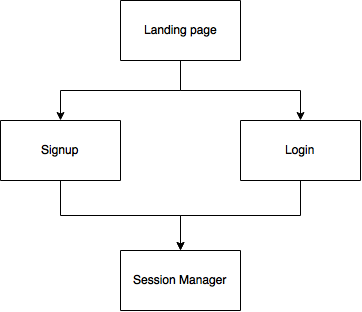
\includegraphics[scale=0.75]{login}
\caption{Authentication control flow}
\label{fig:jsflow}
\end{figure}

\begin{figure}
\centering
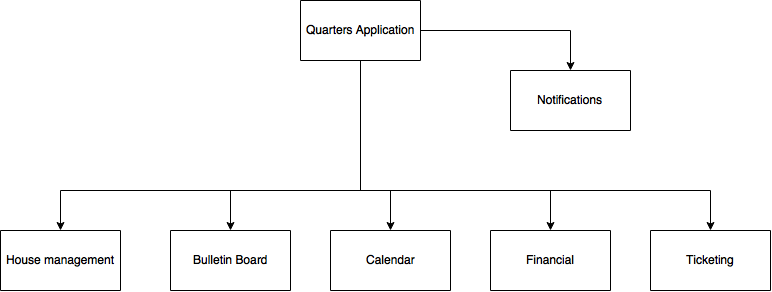
\includegraphics[width=\textwidth]{quarters}
\caption{Demonstrates the flow of requirements within the Javascript modules}
\label{fig:jsflow}
\end{figure}

\end{document}
